\subsubsection{Software methodologies used (D1)}
\label{methodology}

Software development methodology implies the process used for developing particular information systems in a very deliberate, structured, and methodical way. Through this question, we address the fundamental component of development practice in a company. We report the following relevant results:

\begin{itemize}
\item Software development methodologies (Q 6).
\item Requirements gathering (Q 7).
\item Most time-consuming software development activities (Q 8).
\end{itemize}


\paragraph{Software development methodologies}
In our study, as per Figure \ref{fig:methodologies}, we have found that the most popular software development model in Bangladesh is Agile with a response rate of 64\%. The next widely-used model among our respondents is Scrum with a response rate of 46\%. These outcomes match the 2018 Stack Overflow (SO) survey \cite{StackoverflowSurvey2018} result, which reports that Agile and Scrum are the most popular methodologies for developers worldwide keep their projects on track. However, the other methodologies have lower usage rates based on our survey participants: pair programming (20\%), Waterfall (12\%), etc.


\paragraph{Requirements gathering}
The most critical activity that always arises during software development is collecting and analyzing the requirements of a system. Usually, the outcome of the analysis is presented before the client and modified according to their feedback. The more clear and detailed requirements are, the higher the possibility of building software that conducts the client’s anticipation. Corresponding to Figure \ref{fig:requirements}, using plain text (44\%) and storyboard (41\%) are the most widely used requirement gathering techniques among our survey participants. The other relevant techniques include use case (36\%), GUI prototype (35\%), grooming session (30\%), etc. Here we see an appreciable percentage of software practitioners prefer plain text to collect requirements rather than using standard techniques. This is an important finding that requires further analysis for causes and to analyze the potential effects of not practicing standard requirements gathering techniques frequently.

\begin{figure}[h]
\centering
  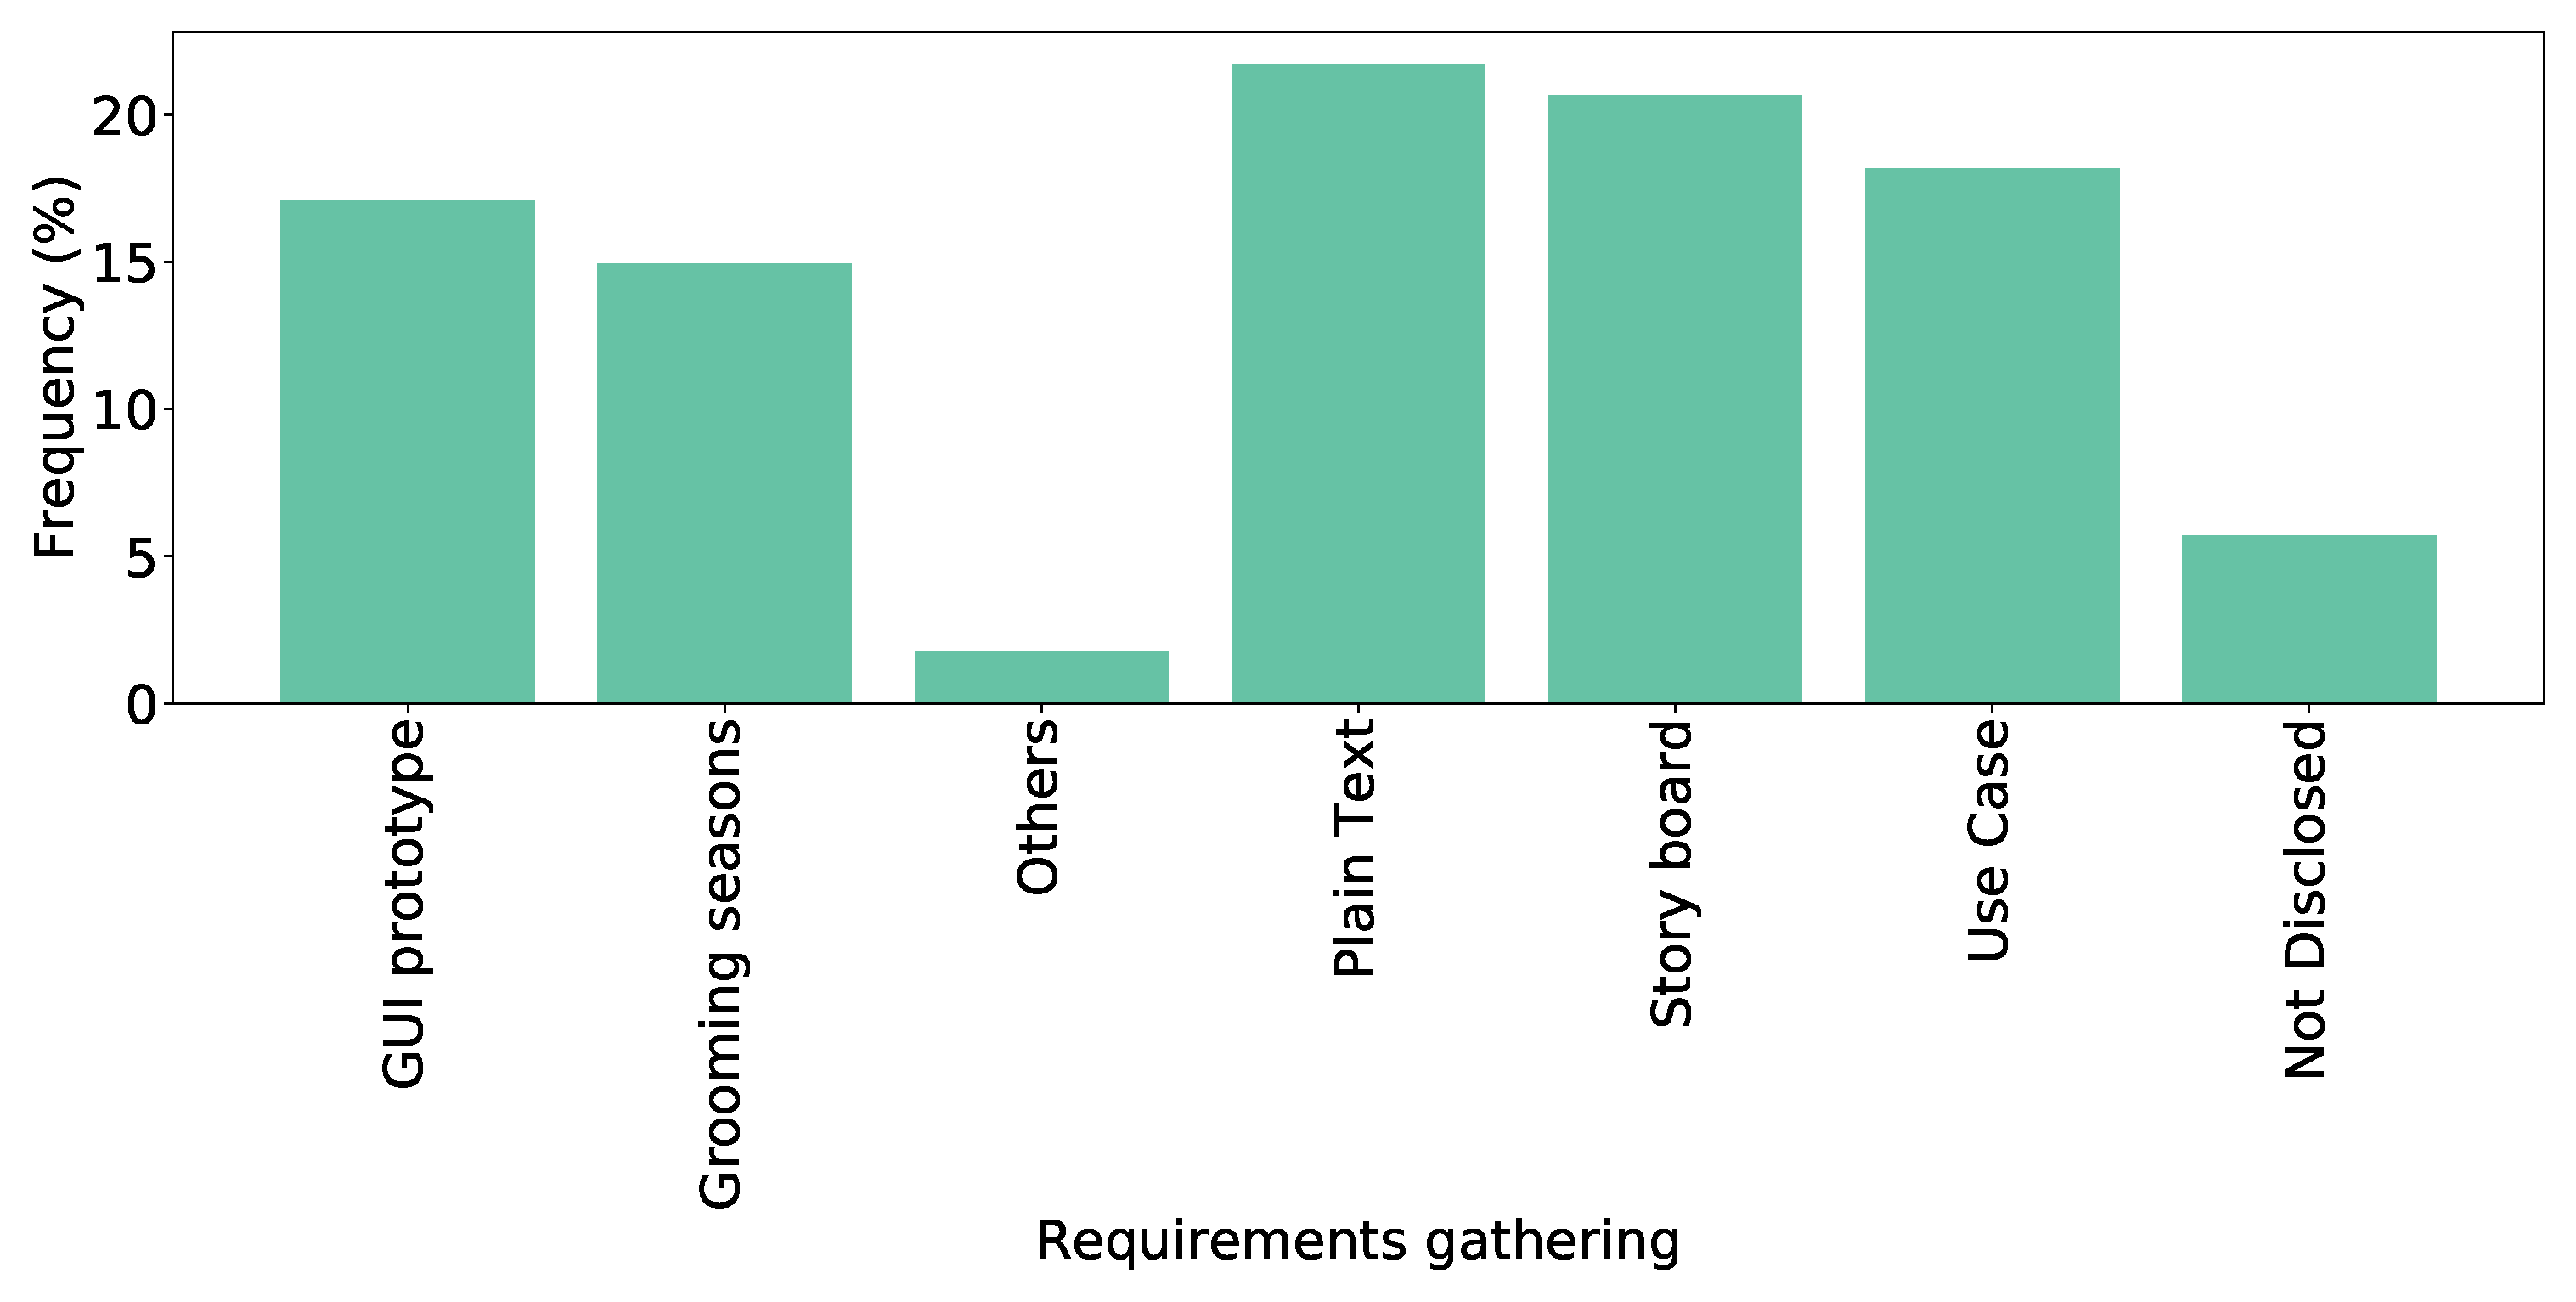
\includegraphics[scale=0.18]{Figures/Requirements_Gathering}
  \caption{Requirements gathering}
  \label{fig:requirements}
\end{figure}


\paragraph{Timeline of Development Activities}
Here, the participants were asked about the most time-consuming software development activities as far as their experience goes. We have presented the activities with respect to the percentage of the participants in Figure \ref{fig:activities}. We see that, according to 65\% of our respondents, most of the time is spent in the implementation stage, whereas the requirement analysis stage requires the second most according to 45\% response. The other usages are program design (37\%), project planning (30\%), testing (19\%), maintenance (17\%), etc.

\begin{figure}[h]
\centering
  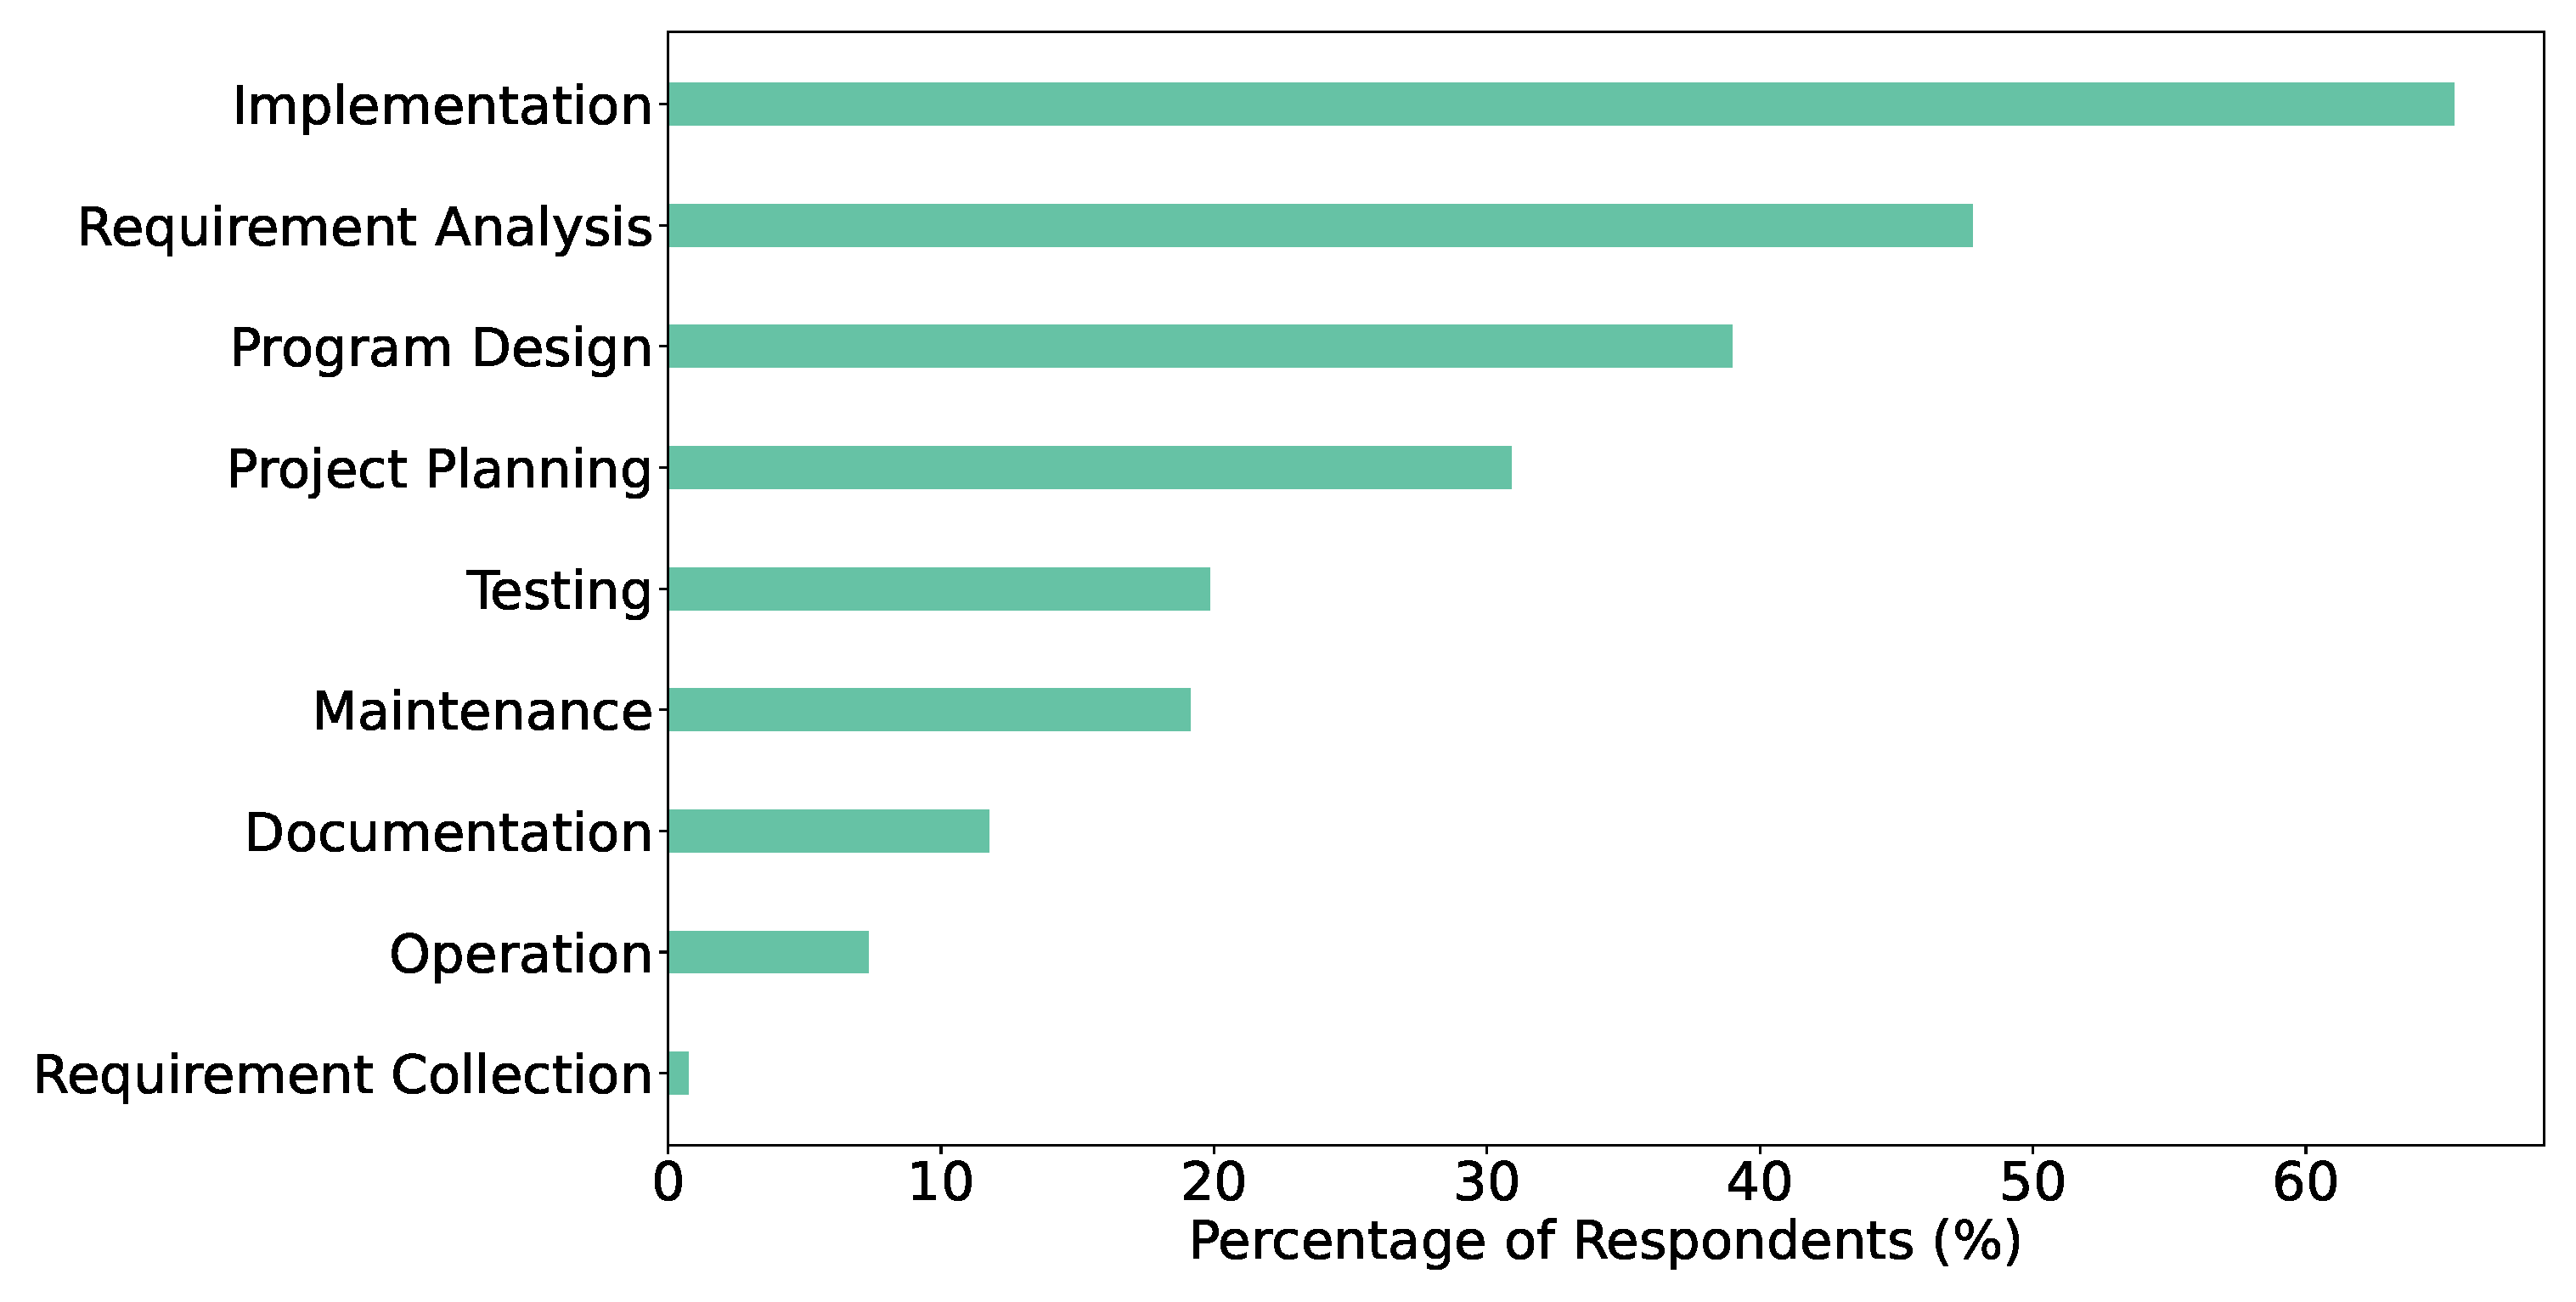
\includegraphics[scale=0.2]{Figures/Respondents_Activities}
  \caption{Software development activities}
  \label{fig:activities}
\end{figure}

We expected that there would be some correlation between software development methodologies (Q6) and the most time-consuming development activities (Q8). Some methodology may add extra time in development activities. Thus we have calculated the Cramér`s V \cite{Cramer1946} between the choice of software development methodologies and most time spent activity of the respondents. Cramér`s V calculates the measure of association between two nominal variables\cite{Sheskin2007}. However, we have not found any significant correlation.

\begin{figure}[h]
\centering
  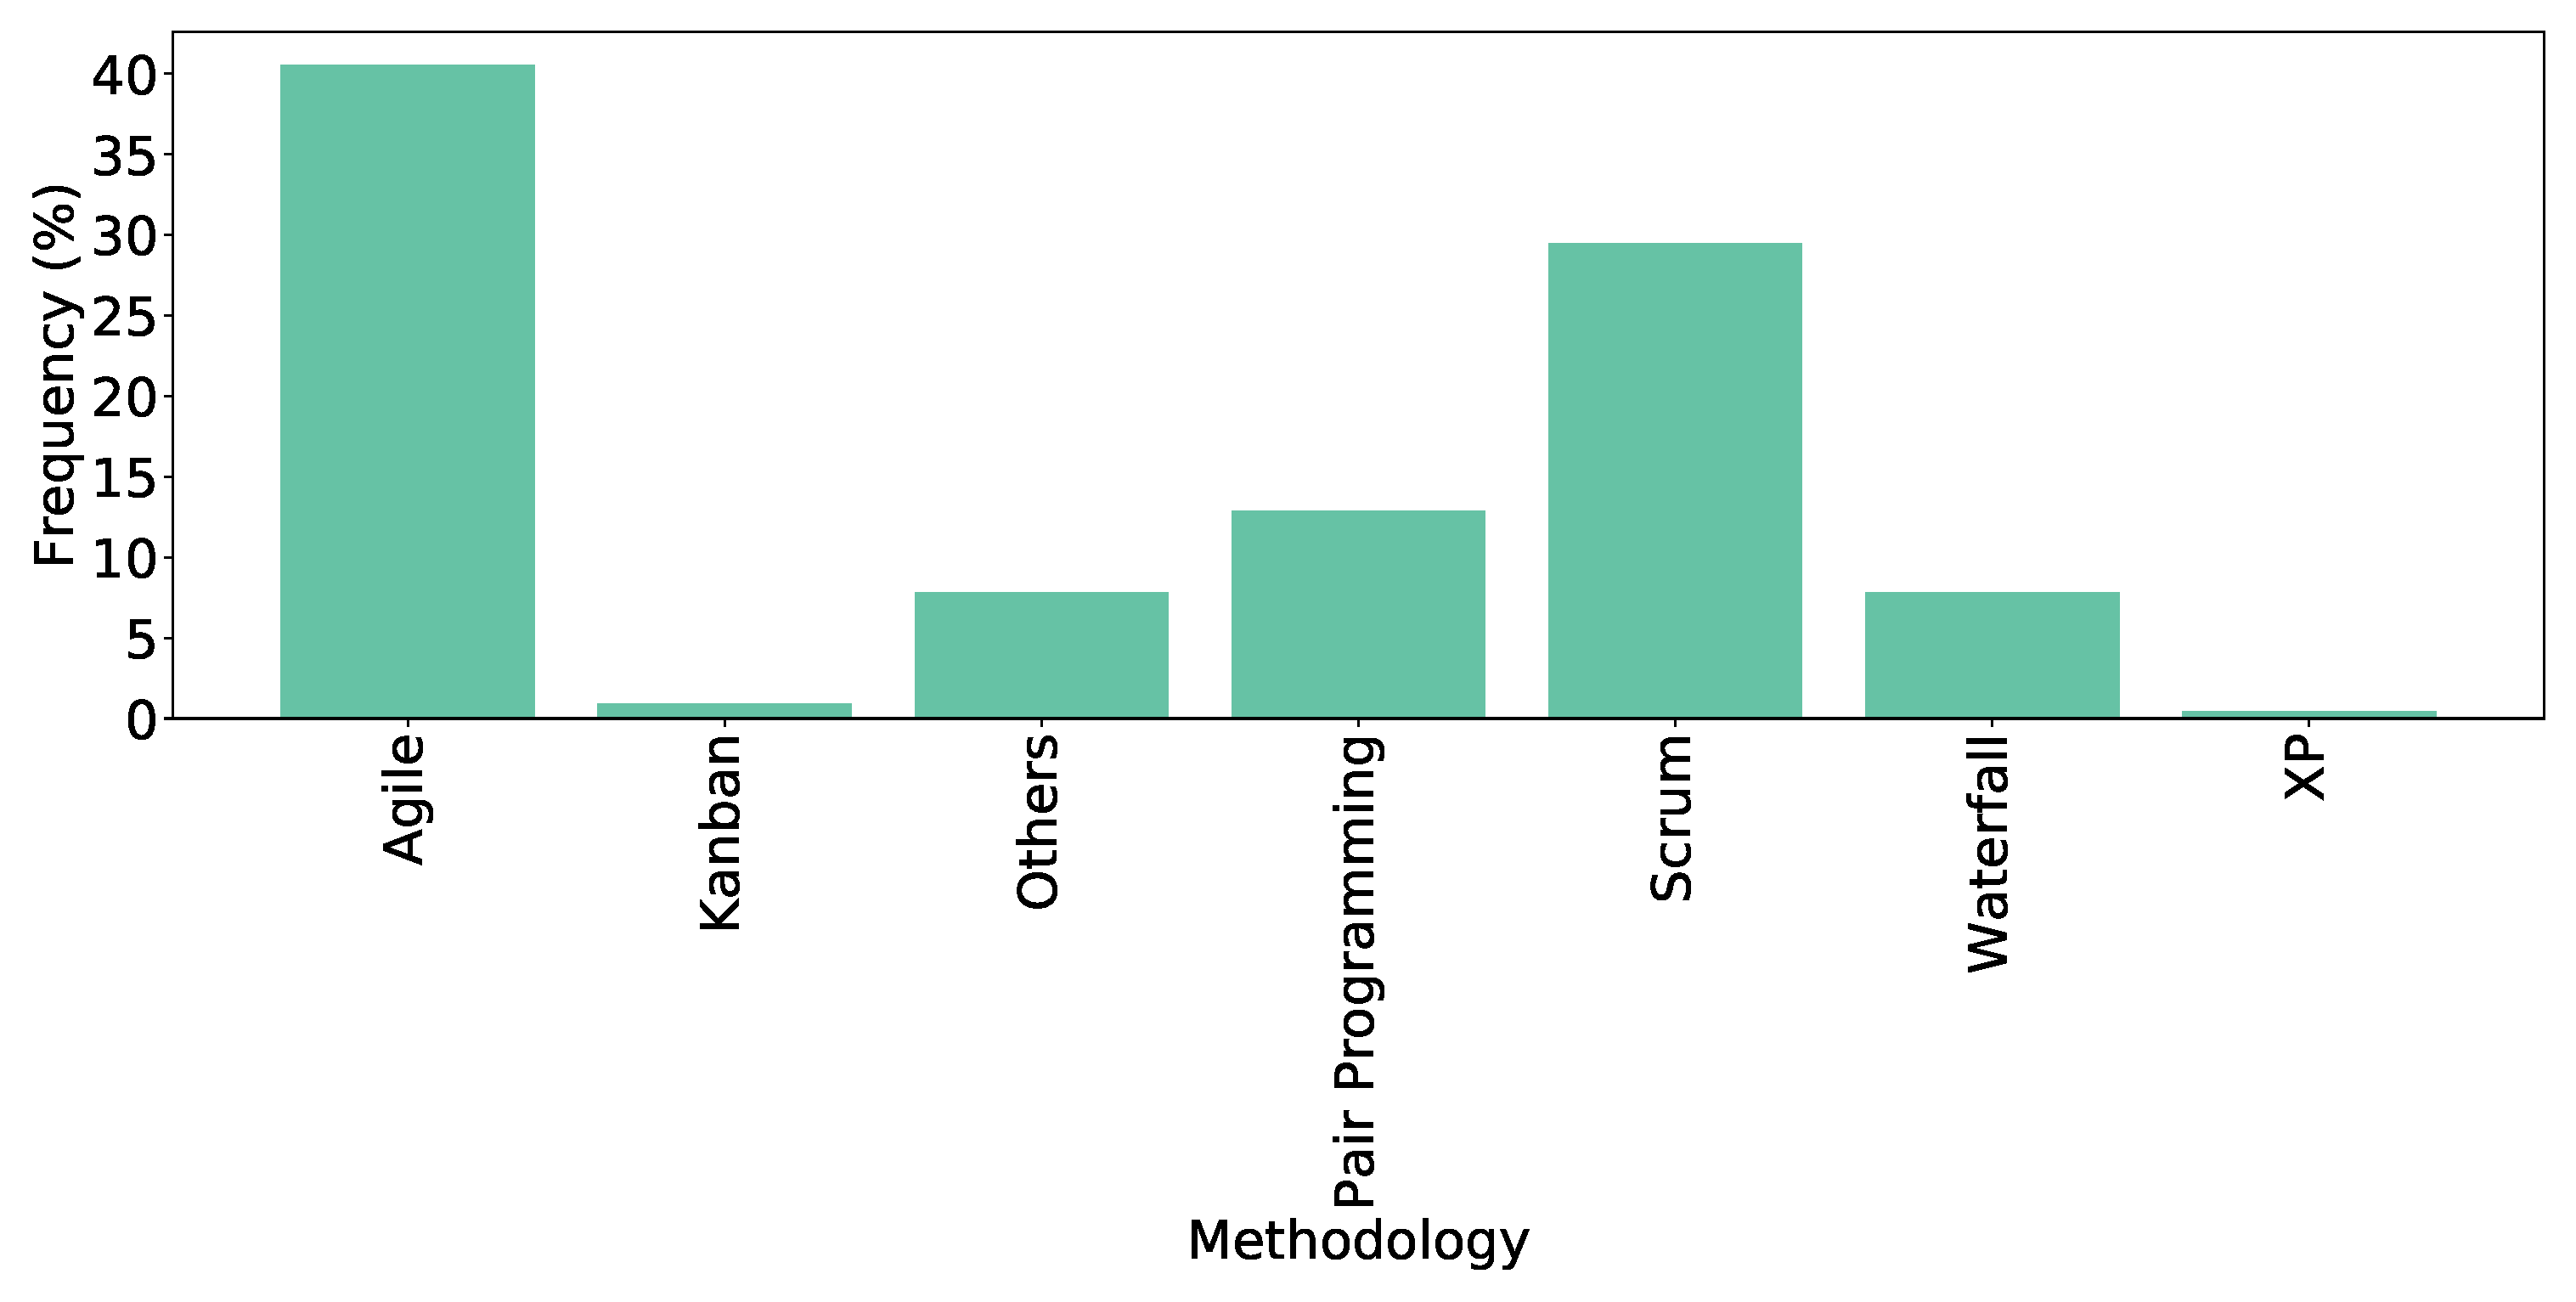
\includegraphics[scale=0.18]{Figures/Respondents_Methodology}
  \caption{Software development methodologies}
  \label{fig:methodologies}
\end{figure}

We guessed that there might be a relation between developers' experience and their activities. It is a general idea that senior developers spend most of their time in requirement specification and design activities, where junior developers spend their time implementing the solution. For analysis purposes, we divided our respondents into two groups based on their professional experience. The two groups are 1) Senior: Developers with more than 5 years of experience 2) Junior: Developers having less than 5 years of experience. We plotted the most time spent activity for the above-mentioned two groups in Figure \ref{fig:activity and seniority}. We can see that our anticipation is right. Junior developers are mostly engaged in the implementation, where senior developers are engaged with requirement specifications.
\anindya{Do you consistently imply coding/development by implementation? In SE, it has a different meaning.}\partha{`Implementation' was one of the options of this closed question. It seems like respondents used it to mean coding/development. One of the responses to another question was `Implementation time carefulness and maintaining a well-developed coding standard.' Though I am not sure, it seems he means coding/development here}

\begin{figure}[h]
\centering
  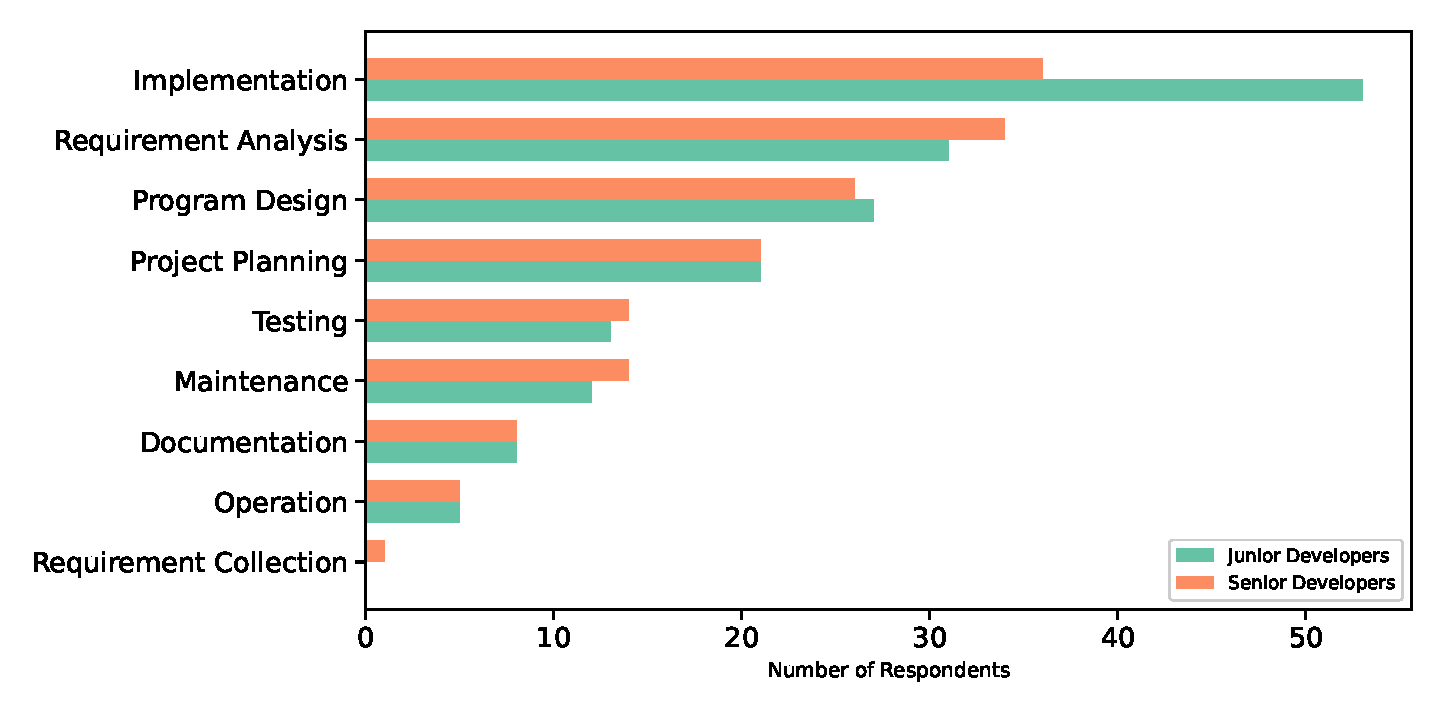
\includegraphics[scale=0.4]{Figures/Activity_and_Seniority.eps}
  \caption{Relation between seniority and activity}
  \label{fig:activity and seniority}
\end{figure}


\boxtext{Developers of the Bangladeshi SE industry generally spend more time on implementation-related activities than planning and testing.}
